% \documentclass[a4paper]{article}
% \usepackage{tikz}

% \begin{document}
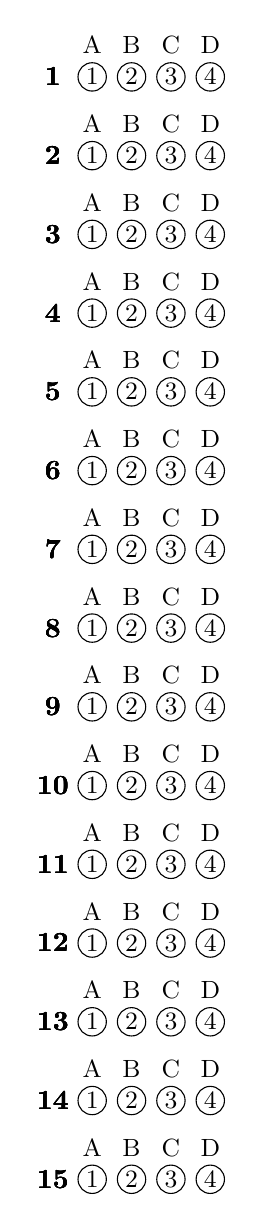
\begin{tikzpicture}[font=\small]
    \foreach \line in {1,2,...,15} {
        \begin{scope}[yshift=-\line cm]
            \foreach \count/\desc in {1/A, 2/B, 3/C, 4/D} { 
                \node at ({\count * 0.5}, 0.4) {\desc};
                \node at (0,0) {\normalsize\textbf{\line}};
                \node[draw,circle,inner sep=1pt] at ({\count * 0.5},0) {\count};
            }
        \end{scope}
    }
\end{tikzpicture}
% \end{document}